\documentclass[]{tufte-handout}

% ams
\usepackage{amssymb,amsmath}

\usepackage{ifxetex,ifluatex}
\usepackage{fixltx2e} % provides \textsubscript
\ifnum 0\ifxetex 1\fi\ifluatex 1\fi=0 % if pdftex
  \usepackage[T1]{fontenc}
  \usepackage[utf8]{inputenc}
\else % if luatex or xelatex
  \makeatletter
  \@ifpackageloaded{fontspec}{}{\usepackage{fontspec}}
  \makeatother
  \defaultfontfeatures{Ligatures=TeX,Scale=MatchLowercase}
  \makeatletter
  \@ifpackageloaded{soul}{
     \renewcommand\allcapsspacing[1]{{\addfontfeature{LetterSpace=15}#1}}
     \renewcommand\smallcapsspacing[1]{{\addfontfeature{LetterSpace=10}#1}}
   }{}
  \makeatother
\fi

% graphix
\usepackage{graphicx}
\setkeys{Gin}{width=\linewidth,totalheight=\textheight,keepaspectratio}

% booktabs
\usepackage{booktabs}

% url
\usepackage{url}

% hyperref
\usepackage{hyperref}

% units.
\usepackage{units}


\setcounter{secnumdepth}{2}

% citations
\usepackage{natbib}
\bibliographystyle{plainnat}

% pandoc syntax highlighting
\usepackage{color}
\usepackage{fancyvrb}
\newcommand{\VerbBar}{|}
\newcommand{\VERB}{\Verb[commandchars=\\\{\}]}
\DefineVerbatimEnvironment{Highlighting}{Verbatim}{commandchars=\\\{\}}
% Add ',fontsize=\small' for more characters per line
\usepackage{framed}
\definecolor{shadecolor}{RGB}{248,248,248}
\newenvironment{Shaded}{\begin{snugshade}}{\end{snugshade}}
\newcommand{\AlertTok}[1]{\textcolor[rgb]{0.94,0.16,0.16}{#1}}
\newcommand{\AnnotationTok}[1]{\textcolor[rgb]{0.56,0.35,0.01}{\textbf{\textit{#1}}}}
\newcommand{\AttributeTok}[1]{\textcolor[rgb]{0.77,0.63,0.00}{#1}}
\newcommand{\BaseNTok}[1]{\textcolor[rgb]{0.00,0.00,0.81}{#1}}
\newcommand{\BuiltInTok}[1]{#1}
\newcommand{\CharTok}[1]{\textcolor[rgb]{0.31,0.60,0.02}{#1}}
\newcommand{\CommentTok}[1]{\textcolor[rgb]{0.56,0.35,0.01}{\textit{#1}}}
\newcommand{\CommentVarTok}[1]{\textcolor[rgb]{0.56,0.35,0.01}{\textbf{\textit{#1}}}}
\newcommand{\ConstantTok}[1]{\textcolor[rgb]{0.00,0.00,0.00}{#1}}
\newcommand{\ControlFlowTok}[1]{\textcolor[rgb]{0.13,0.29,0.53}{\textbf{#1}}}
\newcommand{\DataTypeTok}[1]{\textcolor[rgb]{0.13,0.29,0.53}{#1}}
\newcommand{\DecValTok}[1]{\textcolor[rgb]{0.00,0.00,0.81}{#1}}
\newcommand{\DocumentationTok}[1]{\textcolor[rgb]{0.56,0.35,0.01}{\textbf{\textit{#1}}}}
\newcommand{\ErrorTok}[1]{\textcolor[rgb]{0.64,0.00,0.00}{\textbf{#1}}}
\newcommand{\ExtensionTok}[1]{#1}
\newcommand{\FloatTok}[1]{\textcolor[rgb]{0.00,0.00,0.81}{#1}}
\newcommand{\FunctionTok}[1]{\textcolor[rgb]{0.00,0.00,0.00}{#1}}
\newcommand{\ImportTok}[1]{#1}
\newcommand{\InformationTok}[1]{\textcolor[rgb]{0.56,0.35,0.01}{\textbf{\textit{#1}}}}
\newcommand{\KeywordTok}[1]{\textcolor[rgb]{0.13,0.29,0.53}{\textbf{#1}}}
\newcommand{\NormalTok}[1]{#1}
\newcommand{\OperatorTok}[1]{\textcolor[rgb]{0.81,0.36,0.00}{\textbf{#1}}}
\newcommand{\OtherTok}[1]{\textcolor[rgb]{0.56,0.35,0.01}{#1}}
\newcommand{\PreprocessorTok}[1]{\textcolor[rgb]{0.56,0.35,0.01}{\textit{#1}}}
\newcommand{\RegionMarkerTok}[1]{#1}
\newcommand{\SpecialCharTok}[1]{\textcolor[rgb]{0.00,0.00,0.00}{#1}}
\newcommand{\SpecialStringTok}[1]{\textcolor[rgb]{0.31,0.60,0.02}{#1}}
\newcommand{\StringTok}[1]{\textcolor[rgb]{0.31,0.60,0.02}{#1}}
\newcommand{\VariableTok}[1]{\textcolor[rgb]{0.00,0.00,0.00}{#1}}
\newcommand{\VerbatimStringTok}[1]{\textcolor[rgb]{0.31,0.60,0.02}{#1}}
\newcommand{\WarningTok}[1]{\textcolor[rgb]{0.56,0.35,0.01}{\textbf{\textit{#1}}}}

% longtable

% multiplecol
\usepackage{multicol}

% strikeout
\usepackage[normalem]{ulem}

% morefloats
\usepackage{morefloats}


% tightlist macro required by pandoc >= 1.14
\providecommand{\tightlist}{%
  \setlength{\itemsep}{0pt}\setlength{\parskip}{0pt}}

% title / author / date
\title{Design}
\author{Andrew Grogan-Kaylor}
\date{2019-08-08}

%% -- tint overrides
%% fonts, using roboto (condensed) as default
\usepackage[sfdefault,condensed]{roboto}
%% also nice: \usepackage[default]{lato}

%% colored links, setting 'borrowed' from RJournal.sty with 'Thanks, Achim!'
\RequirePackage{color}
\definecolor{link}{rgb}{0.1,0.1,0.8} %% blue with some grey
\hypersetup{
  colorlinks,%
  citecolor=link,%
  filecolor=link,%
  linkcolor=link,%
  urlcolor=link
}

%% macros
\makeatletter

%% -- tint does not use italics or allcaps in title
\renewcommand{\maketitle}{%     
  \newpage
  \global\@topnum\z@% prevent floats from being placed at the top of the page
  \begingroup
    \setlength{\parindent}{0pt}%
    \setlength{\parskip}{4pt}%
    \let\@@title\@empty
    \let\@@author\@empty
    \let\@@date\@empty
    \ifthenelse{\boolean{@tufte@sfsidenotes}}{%
      %\gdef\@@title{\sffamily\LARGE\allcaps{\@title}\par}%
      %\gdef\@@author{\sffamily\Large\allcaps{\@author}\par}%
      %\gdef\@@date{\sffamily\Large\allcaps{\@date}\par}%
      \gdef\@@title{\begingroup\fontseries{b}\selectfont\LARGE{\@title}\par}%
      \gdef\@@author{\begingroup\fontseries{l}\selectfont\Large{\@author}\par}%
      \gdef\@@date{\begingroup\fontseries{l}\selectfont\Large{\@date}\par}%
    }{%
      %\gdef\@@title{\LARGE\itshape\@title\par}%
      %\gdef\@@author{\Large\itshape\@author\par}%
      %\gdef\@@date{\Large\itshape\@date\par}%
      \gdef\@@title{\begingroup\fontseries{b}\selectfont\LARGE\@title\par\endgroup}%
      \gdef\@@author{\begingroup\fontseries{l}\selectfont\Large\@author\par\endgroup}%
      \gdef\@@date{\begingroup\fontseries{l}\selectfont\Large\@date\par\endgroup}%
    }%
    \@@title
    \@@author
    \@@date
  \endgroup
  \thispagestyle{plain}% suppress the running head
  \tuftebreak% add some space before the text begins
  \@afterindentfalse\@afterheading% suppress indentation of the next paragraph
}

%% -- tint does not use italics or allcaps in section/subsection/paragraph
\titleformat{\section}%
  [hang]% shape
  %{\normalfont\Large\itshape}% format applied to label+text
  {\fontseries{b}\selectfont\Large}% format applied to label+text
  {\thesection}% label
  {1em}% horizontal separation between label and title body
  {}% before the title body
  []% after the title body

\titleformat{\subsection}%
  [hang]% shape
  %{\normalfont\large\itshape}% format applied to label+text
  {\fontseries{m}\selectfont\large}% format applied to label+text
  {\thesubsection}% label
  {1em}% horizontal separation between label and title body
  {}% before the title body
  []% after the title body

\titleformat{\paragraph}%
  [runin]% shape
  %{\normalfont\itshape}% format applied to label+text
  {\fontseries{l}\selectfont}% format applied to label+text
  {\theparagraph}% label
  {1em}% horizontal separation between label and title body
  {}% before the title body
  []% after the title body

%% -- tint does not use italics here either
% Formatting for main TOC (printed in front matter)
% {section} [left] {above} {before w/label} {before w/o label} {filler + page} [after]
\ifthenelse{\boolean{@tufte@toc}}{%
  \titlecontents{part}% FIXME
    [0em] % distance from left margin
    %{\vspace{1.5\baselineskip}\begin{fullwidth}\LARGE\rmfamily\itshape} % above (global formatting of entry)
    {\vspace{1.5\baselineskip}\begin{fullwidth}\fontseries{m}\selectfont\LARGE} % above (global formatting of entry)
    {\contentslabel{2em}} % before w/label (label = ``II'')
    {} % before w/o label
    {\rmfamily\upshape\qquad\thecontentspage} % filler + page (leaders and page num)
    [\end{fullwidth}] % after
  \titlecontents{chapter}%
    [0em] % distance from left margin
    %{\vspace{1.5\baselineskip}\begin{fullwidth}\LARGE\rmfamily\itshape} % above (global formatting of entry)
    {\vspace{1.5\baselineskip}\begin{fullwidth}\fontseries{m}\selectfont\LARGE} % above (global formatting of entry)
    {\hspace*{0em}\contentslabel{2em}} % before w/label (label = ``2'')
    {\hspace*{0em}} % before w/o label
    %{\rmfamily\upshape\qquad\thecontentspage} % filler + page (leaders and page num)
    {\upshape\qquad\thecontentspage} % filler + page (leaders and page num)
    [\end{fullwidth}] % after
  \titlecontents{section}% FIXME
    [0em] % distance from left margin
    %{\vspace{0\baselineskip}\begin{fullwidth}\Large\rmfamily\itshape} % above (global formatting of entry)
    {\vspace{0\baselineskip}\begin{fullwidth}\fontseries{m}\selectfont\Large} % above (global formatting of entry)
    {\hspace*{2em}\contentslabel{2em}} % before w/label (label = ``2.6'')
    {\hspace*{2em}} % before w/o label
    %{\rmfamily\upshape\qquad\thecontentspage} % filler + page (leaders and page num)
    {\upshape\qquad\thecontentspage} % filler + page (leaders and page num)
    [\end{fullwidth}] % after
  \titlecontents{subsection}% FIXME
    [0em] % distance from left margin
    %{\vspace{0\baselineskip}\begin{fullwidth}\large\rmfamily\itshape} % above (global formatting of entry)
    {\vspace{0\baselineskip}\begin{fullwidth}\fontseries{m}\selectfont\large} % above (global formatting of entry)
    {\hspace*{4em}\contentslabel{4em}} % before w/label (label = ``2.6.1'')
    {\hspace*{4em}} % before w/o label
    %{\rmfamily\upshape\qquad\thecontentspage} % filler + page (leaders and page num)
    {\upshape\qquad\thecontentspage} % filler + page (leaders and page num)
    [\end{fullwidth}] % after
  \titlecontents{paragraph}% FIXME
    [0em] % distance from left margin
    %{\vspace{0\baselineskip}\begin{fullwidth}\normalsize\rmfamily\itshape} % above (global formatting of entry)
    {\vspace{0\baselineskip}\begin{fullwidth}\fontseries{m}\selectfont\normalsize\rmfamily} % above (global formatting of entry)
    {\hspace*{6em}\contentslabel{2em}} % before w/label (label = ``2.6.0.0.1'')
    {\hspace*{6em}} % before w/o label
    %{\rmfamily\upshape\qquad\thecontentspage} % filler + page (leaders and page num)
    {\upshape\qquad\thecontentspage} % filler + page (leaders and page num)
    [\end{fullwidth}] % after
}{}

  
\makeatother



\begin{document}

\maketitle



{
\setcounter{tocdepth}{2}
\tableofcontents
}

\hypertarget{color}{%
\section{Color}\label{color}}

\hypertarget{color-model}{%
\subsection{Color Model}\label{color-model}}

\url{https://www.nceas.ucsb.edu/~frazier/RSpatialGuides/colorPaletteCheatsheet.pdf}

\begin{figure}
\centering
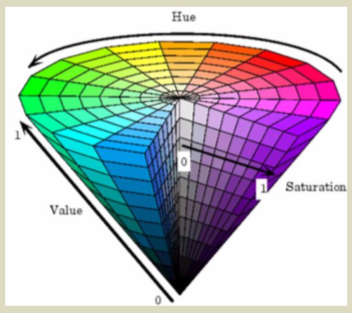
\includegraphics{colorwheel.png}
\caption{color wheel}
\end{figure}

\begin{marginfigure}
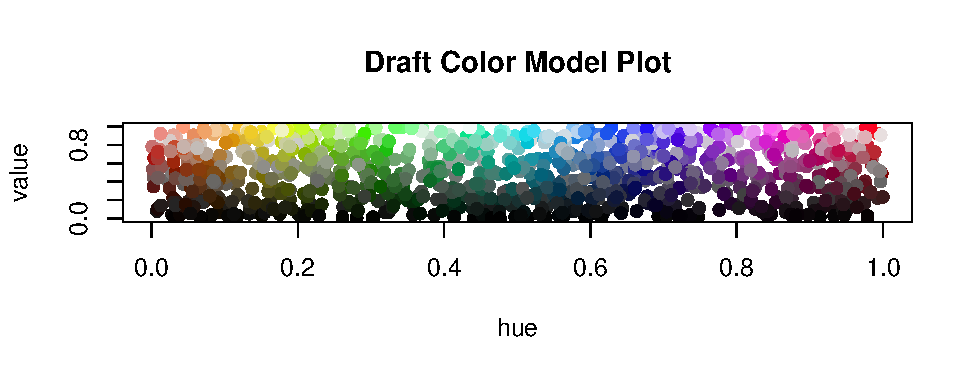
\includegraphics{design_files/figure-latex/unnamed-chunk-1-1} \end{marginfigure}

\hypertarget{unnamed_chunk_1div}{}

You must enable Javascript to view this page properly.

\begin{quote}
R can use many different color models, but often uses a \#\textbf{R}ed,
\textbf{G}reen, \textbf{B}lue model with the amount of each color
indicated in Hexadecimal, 00 to FF, notation.
\end{quote}

\hypertarget{three-types-of-palettes}{%
\subsection{Three Types Of Palettes}\label{three-types-of-palettes}}

\url{http://colorbrewer2.org/}

\begin{Shaded}
\begin{Highlighting}[]
\KeywordTok{library}\NormalTok{(RColorBrewer)}
\end{Highlighting}
\end{Shaded}

\begin{Shaded}
\begin{Highlighting}[]
\KeywordTok{display.brewer.pal}\NormalTok{(}\DecValTok{7}\NormalTok{, }\StringTok{"Set1"}\NormalTok{)  }\CommentTok{# qualitative}
\end{Highlighting}
\end{Shaded}

\begin{marginfigure}
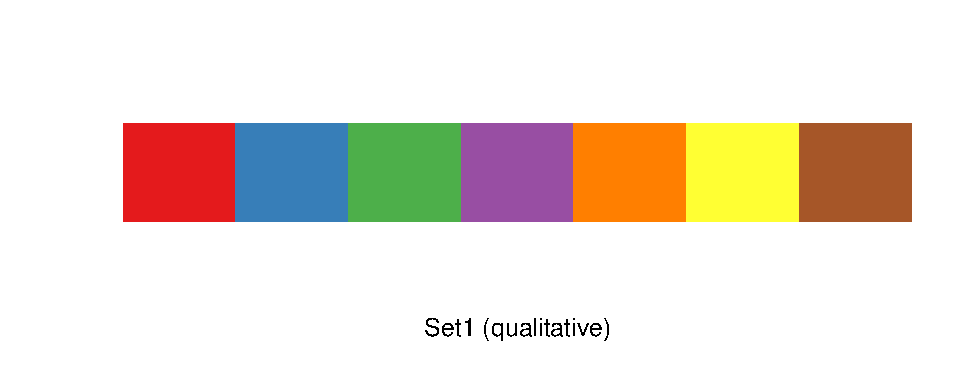
\includegraphics{design_files/figure-latex/unnamed-chunk-3-1} \end{marginfigure}

\begin{Shaded}
\begin{Highlighting}[]
\KeywordTok{display.brewer.pal}\NormalTok{(}\DecValTok{7}\NormalTok{, }\StringTok{"YlOrRd"}\NormalTok{)  }\CommentTok{# sequential}
\end{Highlighting}
\end{Shaded}

\begin{marginfigure}
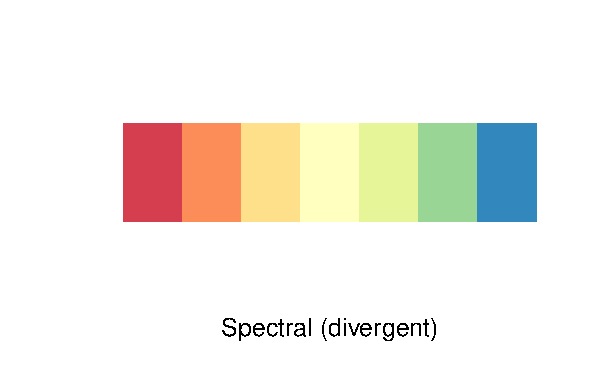
\includegraphics{design_files/figure-latex/unnamed-chunk-4-1} \end{marginfigure}

\begin{Shaded}
\begin{Highlighting}[]
\KeywordTok{display.brewer.pal}\NormalTok{(}\DecValTok{7}\NormalTok{, }\StringTok{"Spectral"}\NormalTok{)  }\CommentTok{# diverging}
\end{Highlighting}
\end{Shaded}

\begin{marginfigure}
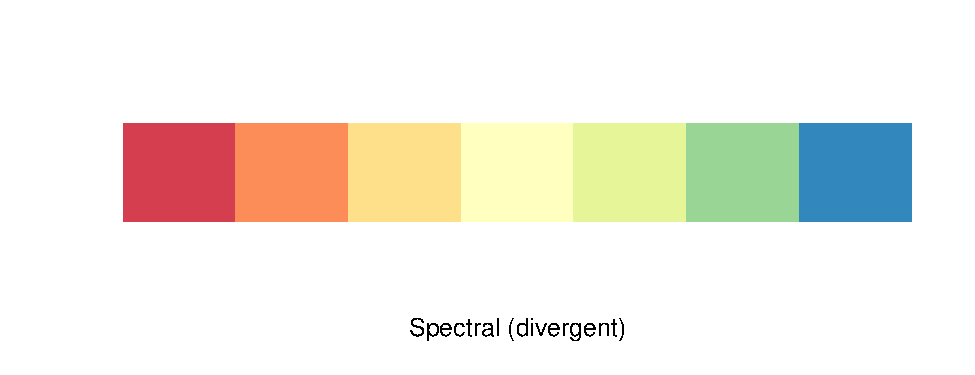
\includegraphics{design_files/figure-latex/unnamed-chunk-5-1} \end{marginfigure}

\begin{Shaded}
\begin{Highlighting}[]
\KeywordTok{display.brewer.all}\NormalTok{()  }\CommentTok{# all palettes}
\end{Highlighting}
\end{Shaded}


\includegraphics{design_files/figure-latex/unnamed-chunk-6-1}

\newpage

\hypertarget{where-do-the-colors-in-ggplot-come-from}{%
\subsection{\texorpdfstring{Where Do The Colors in \texttt{ggplot} Come
From?}{Where Do The Colors in ggplot Come From?}}\label{where-do-the-colors-in-ggplot-come-from}}

Equally spaced around the color wheel.

\begin{figure}
\centering
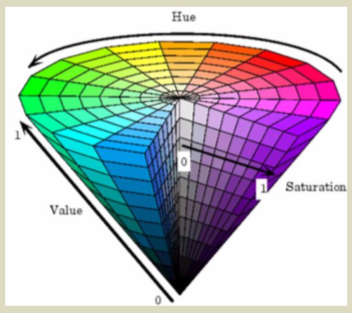
\includegraphics[width=0.2\textwidth,height=\textheight]{colorwheel.png}
\caption{color wheel}
\end{figure}

\begin{Shaded}
\begin{Highlighting}[]
\KeywordTok{library}\NormalTok{(scales)}

\KeywordTok{show_col}\NormalTok{(}\KeywordTok{hue_pal}\NormalTok{()(}\DecValTok{4}\NormalTok{))}
\end{Highlighting}
\end{Shaded}

\begin{marginfigure}
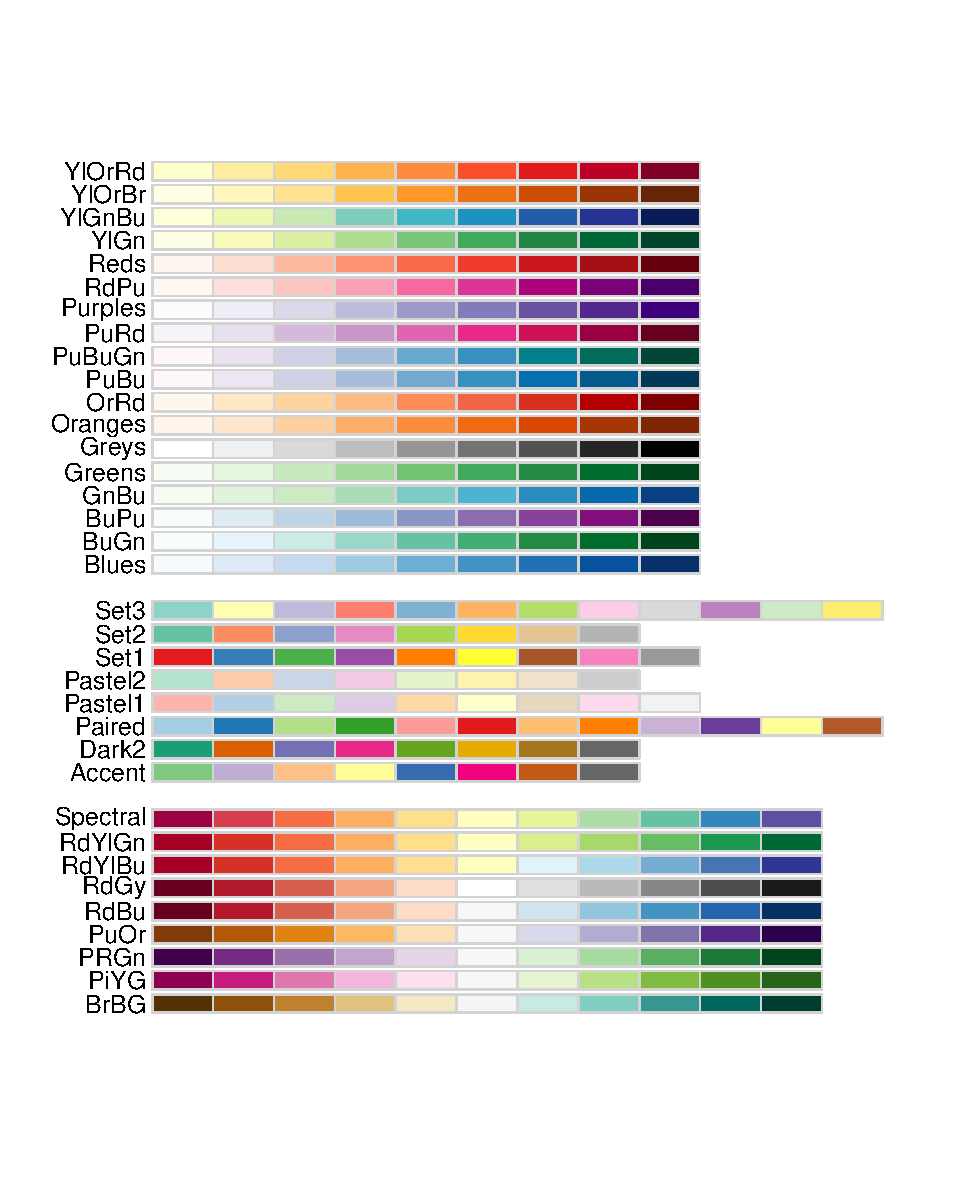
\includegraphics{design_files/figure-latex/unnamed-chunk-7-1} \end{marginfigure}

\hypertarget{many-many-color-options}{%
\subsection{Many Many Color Options}\label{many-many-color-options}}

e.g.~Viridis, which is designed to be \emph{perceptually uniform}.

\begin{marginfigure}

\includegraphics{design_files/figure-latex/unnamed-chunk-8-1} \caption[Viridis Palettes]{Viridis Palettes}\label{fig:unnamed-chunk-8}
\end{marginfigure}

\hypertarget{other-color-and-palette-options}{%
\subsection{Other Color and Palette
Options}\label{other-color-and-palette-options}}

\begin{itemize}
\tightlist
\item
  \url{https://www.garrickadenbuie.com/project/ggpomological/}
\item
  \url{https://bbc.github.io/rcookbook/\#how_to_create_bbc_style_graphics}
\item
  \url{https://github.com/UI-Research/urbnthemes}
\end{itemize}

\hypertarget{fonts}{%
\section{Fonts}\label{fonts}}

\hypertarget{three-major-types-of-fonts}{%
\subsection{Three Major Types of
Fonts}\label{three-major-types-of-fonts}}

\begin{itemize}
\tightlist
\item
  San Serif e.g.~Arial, Helvetica
\item
  Serif Fonts e.g. Times New Roman
\item
  \texttt{Monospaced\ Fonts} e.g. \texttt{Courier} (good for code).
\end{itemize}

\hypertarget{font-rules}{%
\subsection{Font Rules}\label{font-rules}}

\hypertarget{dont-have-too-many-fonts}{%
\subsubsection{\texorpdfstring{Don't have \texttt{too\ many}
fonts!}{Don't have too many fonts!}}\label{dont-have-too-many-fonts}}

\hypertarget{interesting-font-for-heading-standard-font-for-text}{%
\subsubsection{Interesting Font For Heading; Standard Font For
Text}\label{interesting-font-for-heading-standard-font-for-text}}

Interesting Font for Heading

Standard San Serif or Serif Fonts for text. Lorem ipsum dolor sit amet,
consectetur adipiscing elit, sed do eiusmod tempor incididunt ut labore
et dolore magna aliqua. Ut enim ad minim veniam, quis nostrud
exercitation ullamco laboris nisi ut aliquip ex ea commodo consequat.
Duis aute irure dolor in reprehenderit in voluptate velit esse cillum
dolore eu fugiat nulla pariatur. Excepteur sint occaecat cupidatat non
proident, sunt in culpa qui officia deserunt mollit anim id est laborum.

\hypertarget{cognition}{%
\section{Cognition}\label{cognition}}

\hypertarget{dimensions-of-data}{%
\subsection{Dimensions of Data}\label{dimensions-of-data}}

\hypertarget{basic-idea-definition}{%
\subsubsection{Basic Idea / Definition}\label{basic-idea-definition}}

\begin{quote}
\emph{Dimensions} of the Data, \emph{Columns} of the Data,
\emph{Measures}, and \emph{Questions} are all terms essentially pointing
at the same concept.
\end{quote}

\begin{Shaded}
\begin{Highlighting}[]
\KeywordTok{data}\NormalTok{(iris)  }\CommentTok{# iris data set}

\KeywordTok{library}\NormalTok{(DT)  }\CommentTok{# nicely formatted data tables}

\KeywordTok{datatable}\NormalTok{(iris)  }\CommentTok{# dimensions of the data}
\end{Highlighting}
\end{Shaded}

\hypertarget{htmlwidget-0cd13bcaceee80741eed}{}

The \texttt{iris} data set has 5 dimensions Sepal.Length, Sepal.Width,
Petal.Length, Petal.Width, Species.

\hypertarget{species-of-iris}{%
\subsubsection{Species of Iris}\label{species-of-iris}}

Setosa:
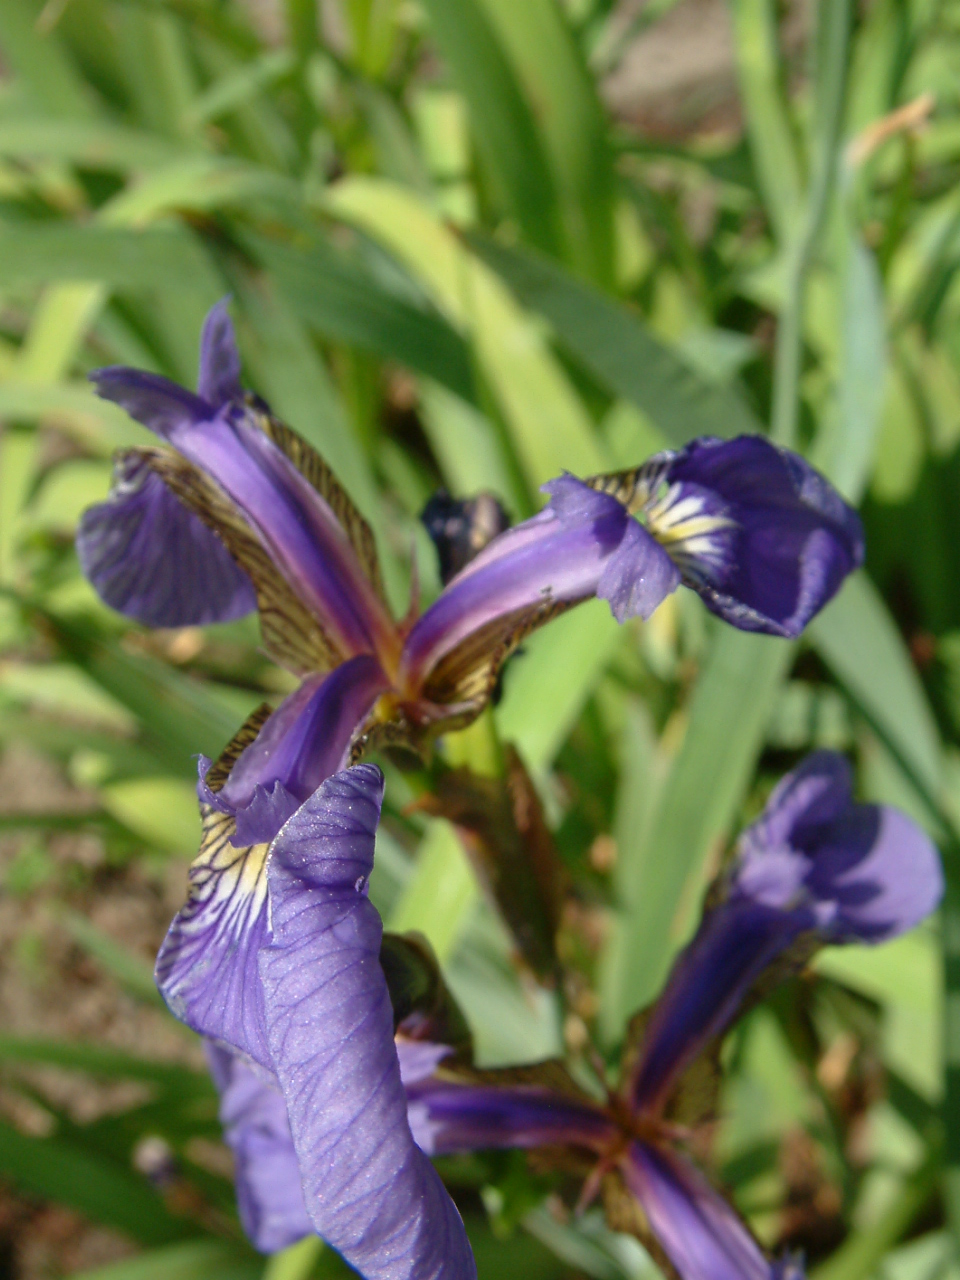
\includegraphics[width=0.2\textwidth,height=\textheight]{Kosaciec_szczecinkowaty_Iris_setosa.jpg}
Versicolor:
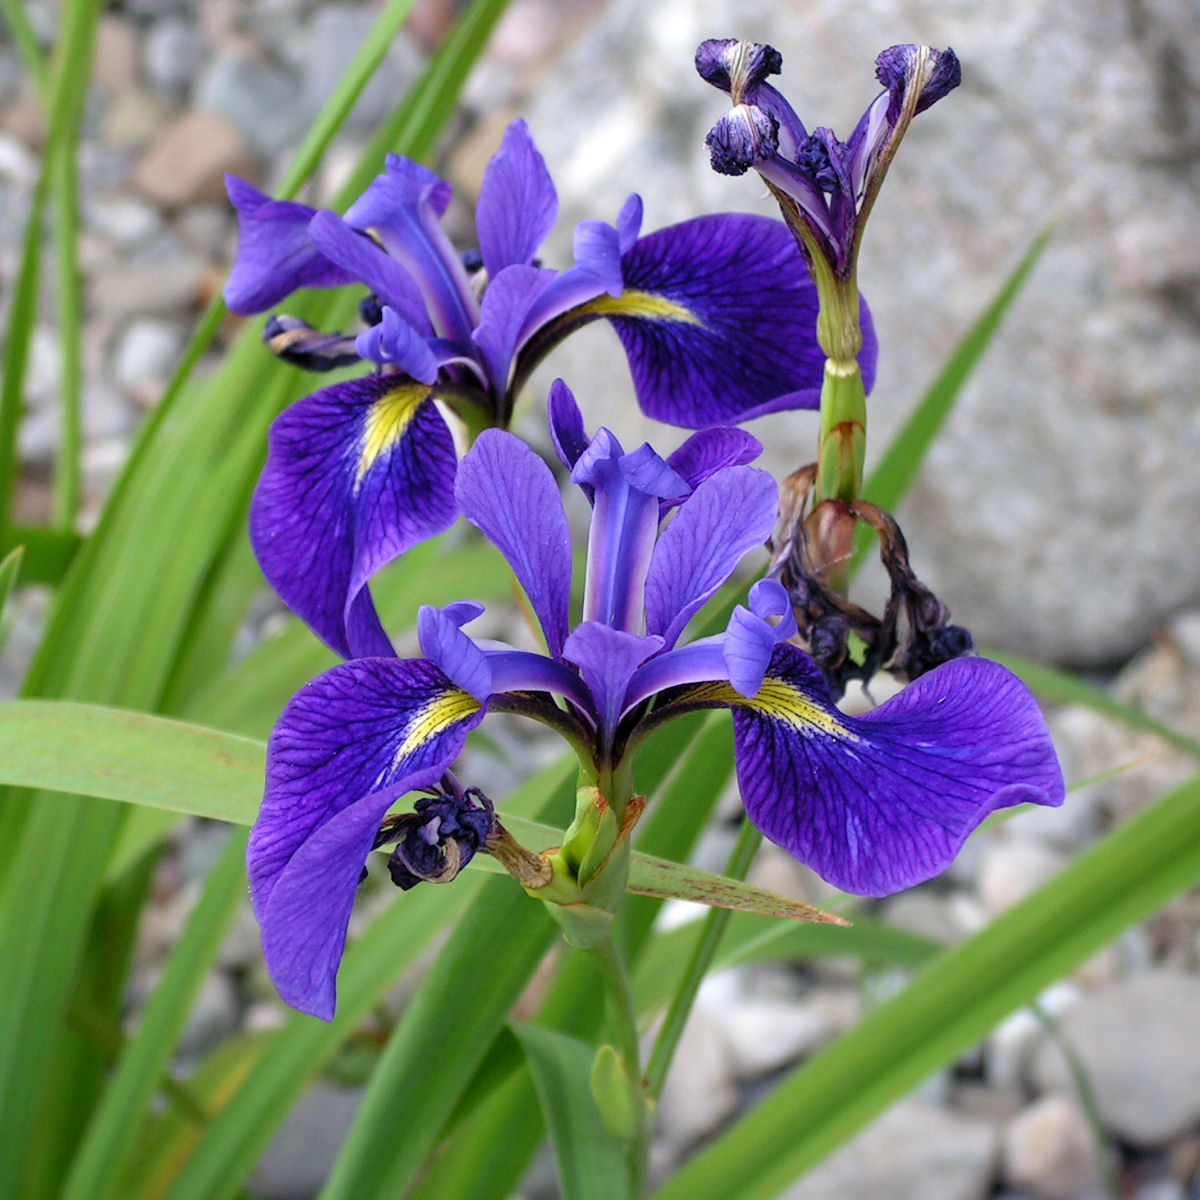
\includegraphics[width=0.2\textwidth,height=\textheight]{Blue_Flag_Ottawa.jpg}
Virginica:
\includegraphics[width=0.2\textwidth,height=\textheight]{Iris_virginica_2.jpg}

\begin{quote}
Iris species images courtesy
\href{https://www.wikipedia.org/}{Wikipedia}.
\end{quote}

\hypertarget{philosophies}{%
\subsubsection{Philosophies}\label{philosophies}}

\begin{marginfigure}
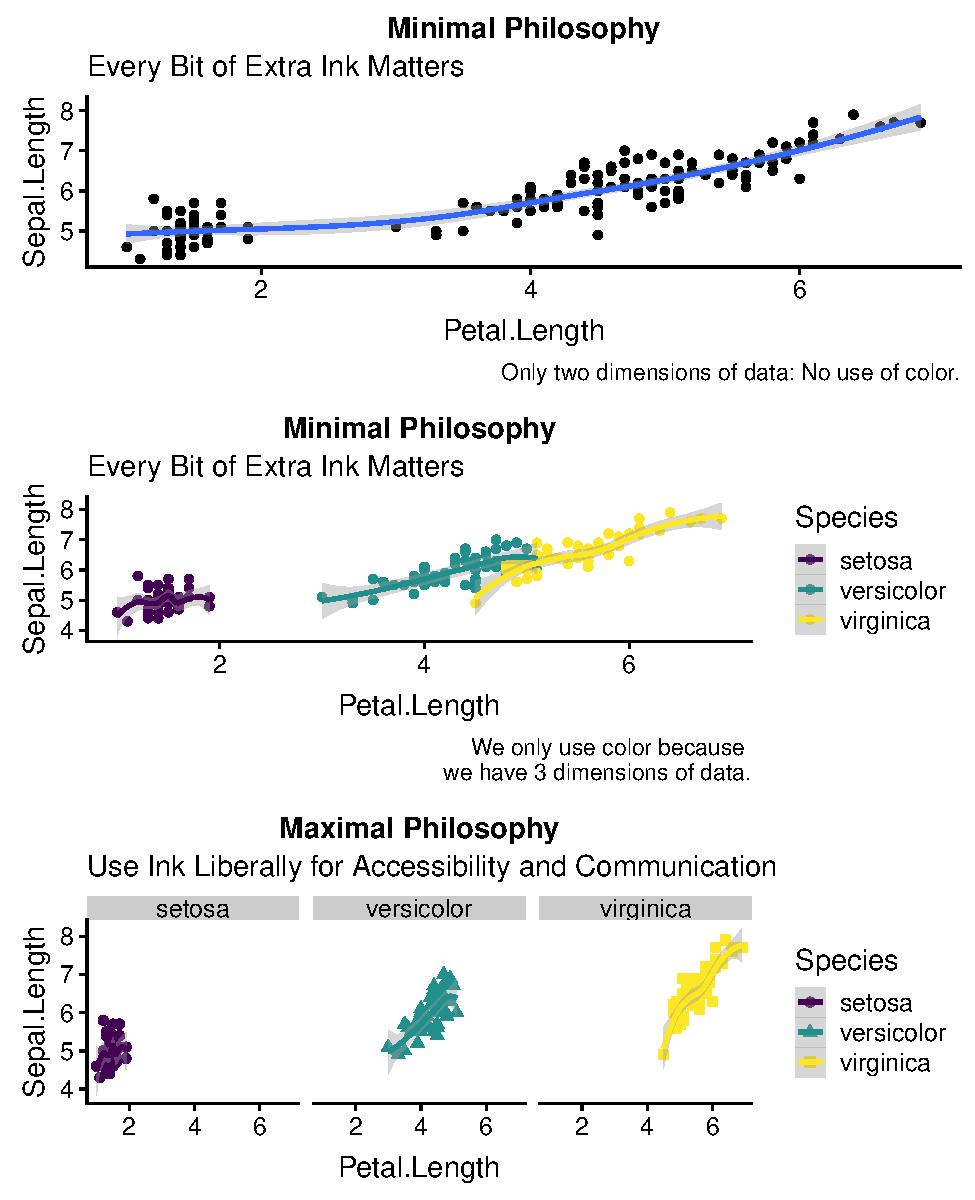
\includegraphics{design_files/figure-latex/unnamed-chunk-10-1} \end{marginfigure}

\hypertarget{some-geometries-are-easier-to-understand-than-others}{%
\subsection{Some Geometries Are Easier To Understand Than
Others}\label{some-geometries-are-easier-to-understand-than-others}}

``Ordering elementary tasks by accuracy \citep{Cleveland1985}:''

\begin{enumerate}
\def\labelenumi{\arabic{enumi}.}
\tightlist
\item
  Position along a common scale
\item
  Position on identical but nonaligned scales
\item
  Length
\item
  Angle \& Slope
\item
  Area
\item
  Volume, Density, Color Saturation
\item
  Color Hue
\end{enumerate}

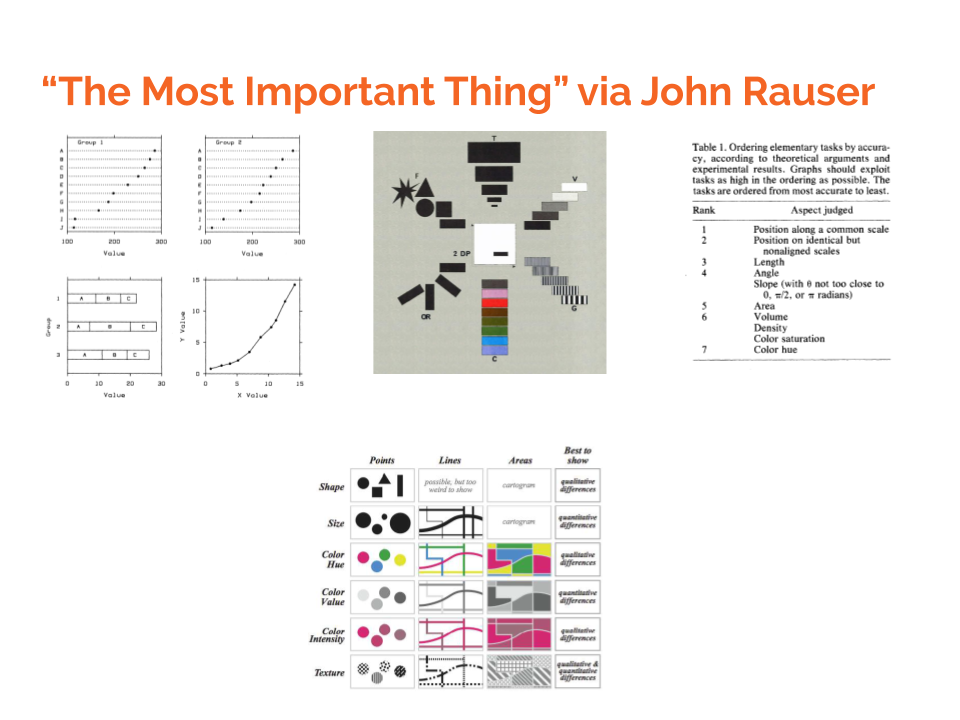
\includegraphics{Rauser-most-important-thing.png}

\bibliography{bibliography.bib}



\end{document}
